\documentclass[tikz]{standalone}
\usetikzlibrary{arrows, calc, decorations.text, positioning}
\begin{document}
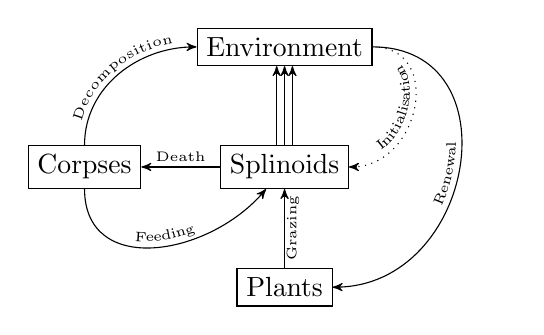
\begin{tikzpicture}[>=stealth',
  every node/.style={draw}
 ]
 \node (E) {Environment};
 \node [below=of E] (S) {Splinoids};
 \node [left=of S] (C) {Corpses};
 \node [below=of S] (P) {Plants};
 
 \draw [<-, dotted, postaction={decorate,decoration={raise=.5ex,text along path,text align=center,text={|\tiny|Initialisation}}}] 
  (S) to [out=0, in=0, looseness = 1.5] (E.east);
  
 \draw [<-, postaction={decorate,decoration={raise=.5ex,text along path,text align=center,text={|\tiny|Renewal}}}]
  (P) to [out=0, in=0, looseness = 1.5] (E.east);
%  \draw [->] (E.east) to [out=0, in=0, looseness = 1] (P);
 
 \draw [<-, postaction={decorate,decoration={raise=.5ex,text along path,text align=center,text={|\tiny|Death}}}]
  (C) to (S);
  
 \draw [->, postaction={decorate,decoration={raise=.5ex,text along path,text align=center,text={|\tiny|Decomposition}}}]
  (C.north) to [out=90, in=180, looseness = 1] (E);
  
 \draw [->, postaction={decorate,decoration={raise=.5ex,text along path,text align=center,text={|\tiny|Feeding}}}]
  (C.south) to [out=270, in=230, looseness = 1.25] (S);
 
 \draw [->, postaction={decorate,decoration={raise=-1ex,text along path,text align=center,text={|\tiny|Grazing}}}] 
  (P) to [out=90, in=270] (S);
 
 \foreach \x in {-1,0,1} {
  \def\dx{.1}
  \draw [->] ($(S.north)+(\dx*\x,0)$) -- ($(E.south)+(\dx*\x,0)$);
 }
\end{tikzpicture}

%    Plant min energy: 12.5664
% Splinoid min energy: 0.0628319
%    Old age duration: 327.114, 117.329, 71.4845
% Starvation duration:
% 	10.2766, 3.686, 2.24575
% 	256.915, 92.15, 56.1438
	
\end{document}
